\documentclass[a4paper]{spie}  %>>> use for US letter paper
%\documentclass[a4paper]{spie}  %>>> use this instead for A4 paper
%\documentclass[nocompress]{spie}  %>>> to avoid compression of citations

\renewcommand{\baselinestretch}{1.0} % Change to 1.65 for double spacing
 
\usepackage{amsmath,amsfonts,amssymb}
\usepackage{graphicx}
\usepackage{todonotes}
\usepackage{lipsum}
\usepackage{pdfpages}
\usepackage[colorlinks=true, allcolors=blue]{hyperref}

\title{Implementation plans for the data reduction pipeline for METIS at the ELT}

\author[a]{Kieran Leschinski}
\author[a]{Hugo Buddelmeijer}
\author[a]{Oliver Czoske}
\author[b]{Gilles Otten}
\author[a]{Martin Balaz}
\author[a]{Fabian Haberhauer}
\author[b]{Jennifer Karr}
\author[c]{Wolfgang Kausch}
\author[d]{Thomas Marquart}
\author[c]{Nadeen Sabha}
\author[b]{Chi-Hung Yan}
\author[c]{Norbert Pryzbilla}
\author[b]{Shiang-Yu Wang}
\author[a]{Werner Zeilinger}

\affil[a]{University of Vienna, T\"urkenschanztra\ss e 18, 1180 Vienna, Austria}
\affil[b]{ASIAA, Taiwan}
\affil[c]{University of Innsbruck, Austria}
\affil[d]{University of Uppsala, Sweden}

\authorinfo{Further author information contact Kieran Leschinski - E-mail: kieran.leschinski@univie.ac.at}

% Option to view page numbers
% \pagestyle{empty} % change to \pagestyle{plain} for page numbers   
\pagestyle{plain}
% \setcounter{page}{301} % Set start page numbering at e.g. 301
 
\begin{document} 
\maketitle

\begin{abstract}


\end{abstract}

% Include a list of keywords after the abstract 
\keywords{ELT, METIS, Data reduction, Pipeline, EDPS, Python, Planning}


\section{Introduction}
% ELT and METIS overview
The ELT (Extremely Large Telescope) will be the largest optical telescope ever constructed, specifically optimized for infrared wavelengths. 
It will feature a 39-meter mirror, collecting light over a nearly 1000-square-meter area. 
Adaptive optic capabilities were integrated into the operational design from the beginning, employing deformable and tip-tilt mirrors within its five-mirror system. 
Such a design will enable the ELT to achieve high Strehl ratio observations (greater than 90\%) at the diffraction limit in mid-infrared wavelengths. 
For instance, a full width at half maximum (FWHM) of 20 milliarcseconds at 3 micrometers and 100 milliarcseconds at 15 micrometers should be achievable by METIS. 
These capabilities will open up countless new parameter spaces in all areas of astronomy and astrophysics

%Overview of METIS

METIS will be the first-light MIR instrument at the ELT.
It will offer  an array of powerful observing modes including  integral-field and long-slit spectrographs, L-M and N-band imagers, and multiple types of coronagraphs for high-contrast imaging and spectroscopy.
Table gives an overview of all the observing modes available with METIS and Brandl et al 2022 <insert refs here> provides a more in-depth description of the current status of the instrument. 

The METIS data reduction pipeline (also referred to as  ``the pipeline'') will play the crucial role of turning usually unintelligible raw data frames into science-grade data products, with which astronomers will be able to unveil the secrets of the cool universe.
Not only are there many observational constrains that the METIS pipeline must deal with, there are also many practical and developmental constraints imposed by the various stake holders associated with the METIS pipeline.

This proceeding paper is split into the following sections. Section \ref{sec:env} will attempt to explain the operational constrains that apply to the development of the METIS pipeline. Section \ref{sec:dev} with present the arguments for developing the pipeline as part of an integrated testing architecture which includes data simulators, archives, and dedicated performance testing frameworks. Details how the pipeline team intends to develop the pipeline given the various operation constraints are given in section \ref{sec:imp}. Section \ref{sec:pip} briefly describes the pipeline topology as detailed in the approved METIS pipeline design documents. Lastly section  \ref{sec:outlook} gives a outlook for the pipeline development out to the initial delivery of the pipeline to ESO in 2028.

Disclaimer: This proceedings paper was written with the help of ChatGPT \footnote{The main intellectual content of the paper belongs solely to the authors, as does the structure of the paper and content of each section and subsection. For each paragraph, the authors wrote down a series of bullet point. ChatGPT was used to string these together into coherent sentences. Ultimately the content and context of each paragraph was checked by the authors to make sure the original intent of the section was conveyed properly. Whether or not this ultimately saved the authors any time is up for debate, but did help with reducing the mental effort of writing the paper.}.

\section{Environmental constraints for the pipeline}
\label{sec:env}

% \begin{itemize}
%     \item - METIS TLR for performance dictate the level to which the METIS pipeline must process data
%     \item - Pipeline is to also support AIV activities
%     \item - Pipeline will need to be able to have functionality available at different levels through out AIV to enable testing
%     \item - AIV team will use pipeline to monitor performance of METIS during the integration phase
%     \item - ESO is expecting METIS to be on-sky for decades, pipeline must work for this length too
%     \item - ESO is rolling out new pipeline tool chains in python: EDPS, PyCPL. This affects the implementation efforts
%     \item - PIP is a very distributed team
% \end{itemize}

\begin{figure}
    \centering
    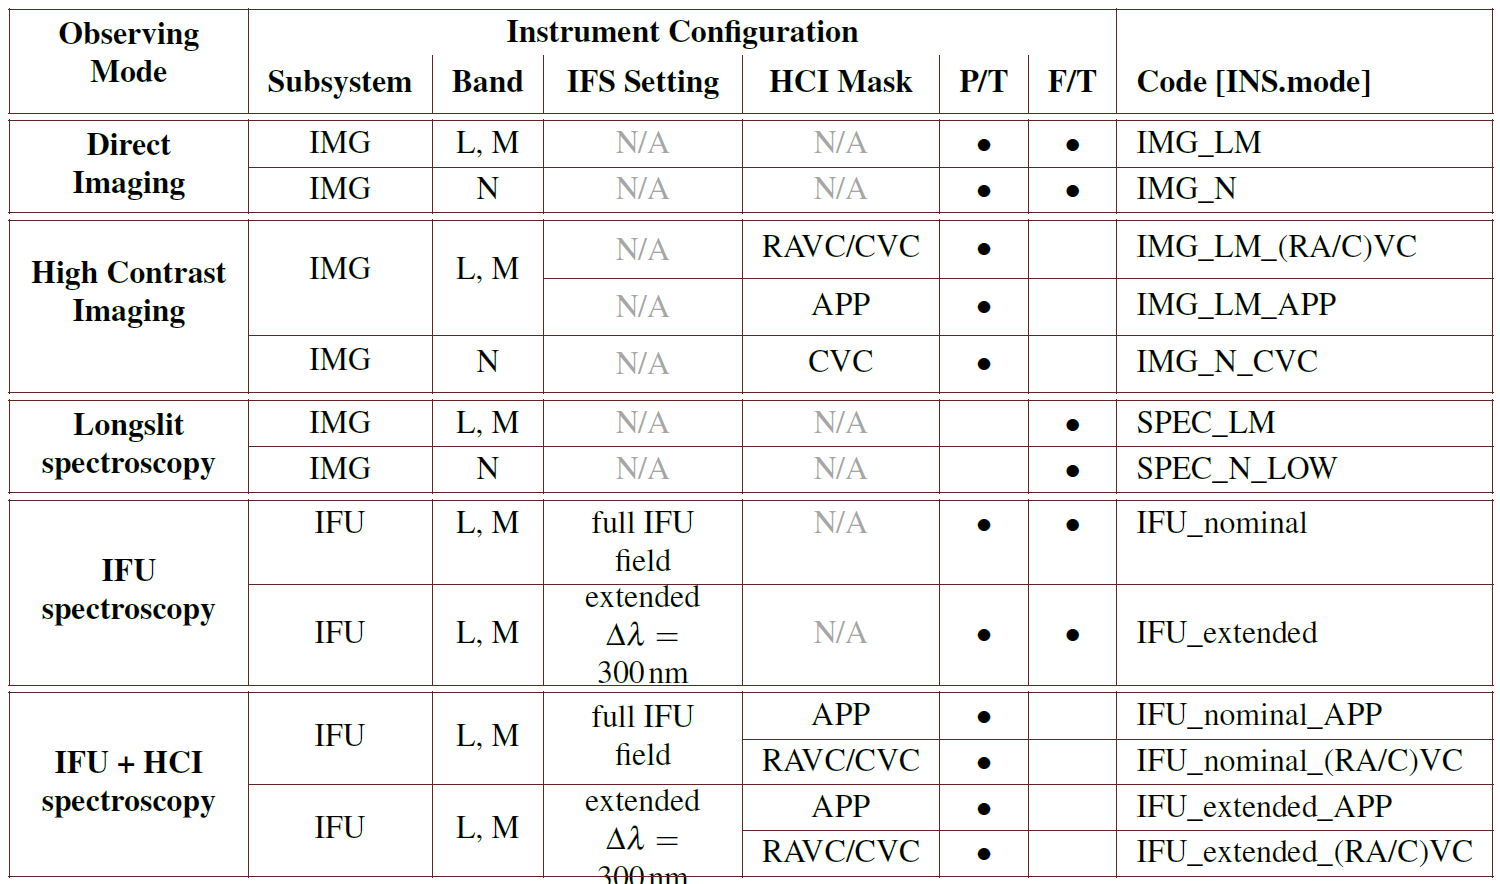
\includegraphics[width=\textwidth]{SPIE_paper/figures/METIS_modes.png}
    \caption{The METIS instrument will include a multitide of observation modes, including standard imaging, long-slit and IFU spectroscopy, and high-contrast modes. The METIS pipeline must be able to handle all of these modes, and indeed also the possibility of multiple modes being used simultaneously. This figure was taken from the latest version (May 2024) of the METIS Data Reduction Library Design document \cite{DRLD}.}
    \label{fig:metis_modes}
\end{figure}


As with every astronomical instrument, METIS is not being built in a vacuum. 
There are many and varied outside factors which influence both the design and the development of the pipeline, from the physical characteristics of the instrument to the external interfaces and frameworks within which the pipeline must operate.

First and foremost, the Top Level Requirements (TLRs) for METIS \cite{ESO-257869} establish the boundary conditions for the METIS pipeline.
These scientific and technical performance requirements will ensuring that the pipeline processes data to the levels necessary for accurate and reliable scientific output. 
The aim of the pipeline team here is to provide a trustworthy tool chain to the astronomical community and to enable a level of scientific discovery worthy of a first-light instrument at the ELT. 

While supporting AIV activities is not an official requirement of the pipeline, it is a useful method to both keep the pipeline development on schedule and keep the functionality aligned with the needs of the instrument. 
The METIS AIV team is expecting to be able to use parts of the the METIS pipeline to monitor and evaluate the instrument's performance.
By leveraging the pipeline, the team will be able to continuously track the behavior of METIS, identify any issues early, and make necessary adjustments . 
This ongoing monitoring is vital for the successful deployment and operation of METIS, ensuring that all components function correctly before the instrument is operational.

During the AIV phase, the pipeline will be required to provide functionality at different levels of readiness to facilitate thorough testing and validation of the instrument. 
To this end the pipeline (and the pipeline team) must remain sufficiently flexible in order to be iterate effectively with the AIV team through out the integration activities.

Considering that the European Southern Observatory (ESO) anticipates METIS to remain on-sky for several decades, the pipeline must be designed for long-term functionality and reliability. 
It should be robust enough to support the instrument throughout its operational life, maintaining high performance and adapting to any future changes or upgrades. 
The longevity of the pipeline is as crucial as the durability of the instrument itself, ensuring sustained scientific productivity.

ESO has recently introduced a new set of python-based tools for developing data reduction pipelines, specifically EDPS \cite{edps} and PyCPL \cite{pycpl}. 
The METIS pipeline team recognises that a python-based tool chain will enable a much greater adoption among the astronomical community, and will (gladly) use the new ESO framework for developling the METIS pipeline. 
Utilizing Python, EDPS, and PyCPL should also help to streamline the development process and ensure future compatibility and support from ESO.
The expected downside to adopting the new python-based framework is the lack of previous experience within the community.
This can however be seen as a hidden opportunity though, as through the inevitable debugging efforts, the METIS pipeline team will also develope a deeper understanding of the ESO packages.

Finally, it is important to note that the pipeline development for METIS involves a highly distributed team. 
A quick look at the author's institutions listed above reveals the geographical diversity of the pipeline team.
Coordinating efforts across different locations and ensuring seamless communication and collaboration is essential for the project's success. 
If leveraged effectively, this diverse range of expertise and perspectives will hopefully significantly enhance the quality and performance of the METIS pipeline.




\section{Need for integrated development and testing architecture}
\label{sec:dev}

% \begin{itemize}
    % \item - Pipeline as a single element in an integrated software ecosystem
    % \item - AIV data archive for storing AIV data and for monitoring the system integration of the METIS instrument
    % \item - AIV system integration tests monitor both functionality and performance of METIS
    % \item - Heavy use of instrument data simulator (ScopeSim) for pre-testing use cases in advance of AIV needs
    % \item - Pipeline as a way of connecting predictions (simulations) to reality
% \end{itemize}


The METIS pipeline functions as a critical component within a sophisticated, integrated software ecosystem. This ecosystem is designed to ensure that all software elements, from data acquisition to processing and analysis, work in harmony. The pipeline's role within this ecosystem is to process and analyze data to meet the rigorous standards set forth in the Technical Level Requirements (TLR). By doing so, it guarantees that the data processed are accurate, reliable, and ready for scientific interpretation.

A vital aspect of the AIV phase is the establishment of an AIV data archive. This archive is tasked with storing all data generated during the AIV activities, serving as a comprehensive repository for integration data. It also provides a crucial platform for monitoring the METIS instrument's integration process. By archiving AIV data, the team can track the instrument's performance over time, quickly identifying and addressing any integration issues that may arise.

The AIV system integration tests are fundamental to ensuring that both the functionality and performance of METIS meet the required standards. These tests rigorously assess the instrument's components, ensuring they function correctly individually and within the larger system. By monitoring both functionality and performance, the AIV team can verify that METIS operates as intended and is prepared for shipment to the ELT.

To prepare for the AIV phase, the team will make extensive use of the instrument data simulator, ScopeSim \cite{scopesim}. This tool allows for pre-testing of various use cases, enabling the team to anticipate and address potential challenges before they arise during actual AIV activities. ScopeSim helps bridge the gap between theoretical predictions and practical implementation, ensuring that the AIV process is as smooth and efficient as possible.

The METIS pipeline serves as a crucial link between simulations and real-world observations. By comparing data processed through the pipeline with simulated data, the team can validate their models and predictions, ensuring that the instrument performs as expected in practice. This capability is essential for confirming the accuracy of simulations and for making any necessary adjustments to enhance the instrument's performance. In this way, the pipeline not only processes data but also helps to refine and validate the scientific models that drive METIS's mission.


\section{Pipeline implementation plans}
\label{sec:imp}

Early on it was decided that the pipeline would support the system-level integration activities.
Practically this means the METIS pipeline should already contain the functionality needed by any system level tests that will use header or pixel data from the METIS detectors.
In order to ensure that this functionality is ready, we plan to make extensive use of simulated data sets. 
Furthermore to aid in continued testing of bother the METIS instrument and the pipeline throughout the full AIV phase, the consortium will store all important data sets from the METIS detectors in an archive.
The following subsections provides a brief overview of how the decision to couple the pipeline development to the AIV activities influences the release schedule of the pipeline.

\subsection{Scheduling matched to AIV plans}
\label{subsec:imp_aiv}

\begin{table}[]
    \centering
\caption{Major METIS AIV milestones for which pipeline recipes need to be ready}
\label{tab:dev_aiv_milestones}
    \begin{tabular}{c|c|l}
    \hline
    \hline
         Date &   METIS AIV phase ID & Description\\
         \hline
         02-2025 &   AIV-010&PIP workstation setup in Leiden\\
         11-2025 &   AIV-250&Dress-rehearsal of data flow chain\\
 02-2026 & AIV-370&IFU system testing\\
 10-2026 &  AIV-490&IMG/LSS system testing\\
 12-2027 & AIV-640&Preliminary acceptance Europe (PAE)\\
 12-2028 & AIV-920&Commissioning on-sky at ELT starts\\
 \hline
 \end{tabular}
      
\end{table}

Table \ref{tab:dev_aiv_milestones} lists the major AIV testing phases when the AIV team will require functional aspects of the pipeline. 
As the integration activities progress and more sub-systems are integrated into the cryostat, so too with the demand for pipeline functionality grow. 
The pipeline development schedule has been designed to move in lock-step with the AIV integration schedule.
This schedule implies a very tight development timeline for the pipeline team.
While attempting to reconcile the available person-power in the pipeline team with the needs of the AIV schedule we recognised that not all AIV tests need fully functioning pipeline recipes. 
We therefore decided to split the development of each pipeline recipe into four levels in order to accommodate the tight timeline dictated by AIV activities.
The different levels of development are described in more detail in section \ref{subsec:imp_levels}.
A brief overview of the AIV phases and the requirements on the pipeline is as follows:

\begin{itemize}
    \item \textbf{AIV-010, PIP workstation setup} : At the beginning of the AIV activites the pipeline workstation will be installed in the AIV Hall in Leiden. A working pipeline skeleton is required to test the interfaces to other subsystems, most notably the staging area for freshly data frames from the METIS detectors. 
    \item  \textbf{AIV-250, Dress-rehearsal of data flow chain} : This phase foresees the integration of the IFU optics into the cryostat, excluding the detectors. This will be the first time the full data flow system - from raw detector readouts through to processed files - is tested. Recipes for the IFU data reduction must be ready at the functional level by this stage.
    \item \textbf{AIV-370, IFU system testing} : The IFU module will be fully mated with the detectors and the instrument will be cooled to operating temperature. The phase includes all lab-based performance tests for the IFU module. All IFU-pipeline recipes will need to be available (mostly) at the performance level in order for the AIV team to test the perfomance of the IFU module against the top level requirements.
    \item \textbf{AIV-490, IMG/LSS system testing} : The imaging and long-slit sub-system, including HAWAII and GeoSnap detectors, will have been integrated into the cryostat by this stage and performance testing as a whole instrument will begin. All imaging and long-slit recipes used by the lab-based performance tests (i.e. utilising the warm calibration unit) will need to be at the performance level, while recipes that require on-sky observations (e.g. telluric corrections) may remain at the functional level.
    \item \textbf{AIV-640, Preliminary acceptance Europe (PAE)} : PAE represents the end of the main pipeline development stage. As such all recipes, including those that will only be fully tested on-sky, must be at the performance level. Heavy use will be made of the instrument data simulator in order to achieve this.
    \item \textbf{AIV-920, Commissioning on-sky at ELT starts} : Initial data from on-sky observations at the ELT will allow the pipeline team to test the performance of the data reduction recipes against the top level requirements for scientific output. Recipes which allow METIS to meet its required performance will be receive the classification of science-grade. Effort will then be spent on upgrading the algorithms in the recipes which don't deliver data compliant with the TLRs.
\end{itemize}


\subsection{Functionality levels}
\label{subsec:imp_levels}

The development of each software recipe for the METIS data reduction pipeline is structured into four distinct phases: skeleton, functional, performance, and science-grade. This phased approach allows for targeted progress, ensuring that development can pause once the software meets the requirements for any upcoming Assembly, Integration, and Verification (AIV) system functional or performance tests. By structuring development in this way, team members can efficiently move between multiple software recipes, focusing their efforts where they are most needed and avoiding the inefficiencies that can arise from getting bogged down in overly detailed or premature optimizations. This strategy ensures a balanced and flexible development process, maximizing productivity and maintaining alignment with project milestones. 
  
 \begin{enumerate}
     \item \textbf{Skeleton recipes }are the initial stage in the development of each software recipe for the METIS data reduction pipeline. During this phase, the software recipes are essentially barebones structures that primarily focus on handling file input and output operations correctly. Despite their minimal functionality, these recipes adhere to the output specifications outlined in the design document and are capable of reading the necessary metadata from input files. Furthermore, the recipes are designed to reject or fail gracefully if inappropriate files are used as input, ensuring robustness and reliability from the outset. This foundational phase sets the stage for more advanced development, providing a clear framework that supports subsequent enhancements in functionality and performance.
 
     \item \textbf{Functional recipes} build upon the skeleton phase by incorporating sufficient code to fulfill the primary tasks outlined in the design document for each software recipe. In this phase, the recipes not only manage file input and output but also perform their intended functions, although they may not yet handle all edge cases. The pixel values in the output should reflect an initial, first-order correction, providing a meaningful representation of the data. Additionally, the internal structure of the recipes is designed to facilitate further development and expansion in later phases. Comprehensive documentation for each function should be available, and unit tests should utilize simulated data products to verify that the recipes perform their designated tasks correctly. This phase ensures that the core functionality is in place and ready for refinement and optimization in subsequent stages. 

     \item \textbf{Performance recipes} will have reached an advanced stage of development. They incorporate all expected functionalities and can handle various edge cases encountered during scientific operations. These recipes are designed to process raw data to meet the performance standards defined in the METIS science top-level requirements. However, testing is limited to simulated data and data collected during AIV testing runs. While this approach allows for thorough lab testing, it does not replicate all potential challenges encountered during actual observations. Nonetheless, achieving performance-level recipes represents significant progress toward readiness for deployment with the METIS instrument on the Extremely Large Telescope. 

     \item \textbf{Science-Grade recipes}: In an ideal scenario, science recipes would mirror the capabilities of performance recipes, as thorough lab testing would have accounted for all possible edge cases. However, the reality of on-sky testing during the METIS commissioning run may unveil unexpected challenges. This could necessitate upgrades or even complete redesigns of various algorithms to ensure optimal performance in real-world conditions. A recipe will only earn the classification of ``science grade'' once it has undergone testing with on-sky data, and the resulting reduced data products align with the scientific performance targets outlined in the METIS Top-Level Requirements (TLRs). This iterative process underscores the importance of rigorous testing and adaptation to ensure that METIS can deliver scientifically meaningful results once operational. 
 \end{enumerate}


\subsection{Integration with data simulator}
\label{subsec:imp_sim}

\missingfigure




\subsection{Development tools}
\label{subsec:imp_tools}
ESO has shown a commitment over the last several years to move its data reduction pipeline towards a new system based on python. 
This is evident in the recent release of the EDPS \cite{edps} and PyCPL \cite{pycpl} packages.
These two packages are meant as replacements for the existing EsoRex and CPL systems written in C.
Given these developments, we took the decision to implement the METIS pipeline primarily in Python.
Although Python is not known for it's computation speed, it does have several advantages in terms of reducing the time needed by developers to code the pipeline as well as providing developers with easy-to-use debugging tools. 
Because of these benefits we anticipate a reduction in the time and effort needed to develop the METIS pipeline.
Additional benefits include the possibility of forking third-party python repositories and reusing already existing code for any of the tasks that are not included in the ESO stack (CPL and HDRL). 
Example of packages which may provide such functionality to the METIS pipeline include: TIPTOP \cite{tiptop}, HEEPS \cite{HEEPS} and PyREDUCE \cite{pyreduce}

In addition to the use of the python ecosystem, we are taking advantage of the tool chain provided by Github. 
These extra tools significantly aid in the development and management of the pipeline beyond the core version control capabilities of Git. 
We use the GitHub Issues and Projects for tracking and managing tasks, bugs, and feature requests. 
Github-Issues have sofar helped us overcome the tyranny of distance in our distributed team be allowing specific tasks to be assigned to members and linked to specific parts of the project. 
This has given us a clear and organized way to manage and trace work. 
We are also using the Github-Projects feature to visualize and manage the development workflow. 
This makes it easier to see the status of tasks at a glance and ensure the pipeline development stay on track.

We take full advantage of are the GitHub Actions service too. 
Github Actions allow us to automate the Continuous Integration process for the development of the pipeline. 
This automation should enhance code quality and speed up the development cycle by ensuring the test suite is run every time a pull request is made. 

Finally pull requests are the main way for us to conduct the all important step of reviewing each others code. 
They allow us to propose changes to the codebase, discuss those changes with other team members, and conduct thorough reviews before merging. 
By doing so we aim to maintain a high standard of code quality despite very few chances for physical interaction and discussions in person.

So far these the pipeline team, distributed over 4 institutes globally, has been able to work very closely and effectively. 
Time will tell whether the echos of the Covid era will prove the distributed-team model for software development to be as effective as the legacy co-location development model.


\subsection{Release schedule}
\label{subsec:imp_schedule}

The delivery schedule during the pipeline development stage is set by the ESO standards document for data flow deliveries \cite{1618}. 
This dictates that the pipeline team (unless otherwise agreed) will deliver and updated version of the data reduction library (DRL) every three months starting 12 months after the final design review and extending until the pipeline is officially accepted by ESO.
The first release of a full pipeline is expected at the milestone for ``Preliminary Acceptance Europe''.
The devil is in the detail though.
The definition of a ``full'' pipeline does not necessarily mean a finished pipeline.
A ``full'' pipeline refers to a pipeline which

\begin{table}[]
\caption{Release schedule for the METIS data reduction pipeline software.}
\label{tab:pip_releases}
\begin{tabular}{|lcllll|}
\hline
Year & Date & Version & Version description & AIV-Phase & Nearest METIS Milestone          \\
\hline
\hline
{2024}          & 15. Nov.      & v0.1             & ESO : Skeleton functional      &                                        & ESO 1st pipeline skeleton delivery   \\
\hline
{2025}          & 15. Feb.      & v0.2             & AIV-A: Skeleton integrated    & 10                 & AIV Hall PIP workstation integration \\
                                  & 15. Mai       & v0.2.1           & AIV-A: Skeleton engineering  &                                        &                                      \\
                                  & 15. Aug.      & v0.2.2           & AIV-A: Skeleton LMS           &                                        &                                      \\
                                  & 15. Nov.      & v0.2.3           & AIV-C : LMS functional       & {250}                & LMS Cold Functional test             \\
\hline
{2026}          & 15. Feb.      & v0.3             & AIV-D : LMS performance       & {370}                & Instrument verification C/D          \\
                                  & 15. Mai       & v0.3.1           & AIV-D : LMS updates 1         &                                        &                                      \\
                                  & 15. Aug.      & v0.3.2           & AIV-D : LMS updates 2        & {350}                & IMG Cold Functional test             \\
                                  & 15. Nov.      & v0.4             & AIV-E : IMG functional         & {490}                & Instrument verification E            \\
\hline
{2027}          & 15. Feb.      & v0.4.1           & AIV-E : LSS functional      &                                        &                                      \\
                                  & 15. Mai       & v0.4.2           & AIV-E : IMG+LSS performance   &                                        &                                      \\
                                  & 15. Aug.      & v1.0             & ESO : Full pipeline PAE         & {650}                & PAE testing                          \\
                                  & 15. Nov.      & v1.0.1           & PAE : updates 1              &                                        &                                      \\
\hline
{2028}          & 15. Feb.      & v1.0.2           & PAE : updates 2               &                                        &                                      \\
                                  & 15. Mai       & v1.1             & Armazones : update 1           & {850}                & Cold Check-in test Chile             \\
                                  & 15. Aug.      & v1.1.1           &Armazones : update 2          &                                        &                                      \\
                                  & 15. Nov.      & v1.2             & ESO : Full pipeline PAC         & {940}                & PAC Testing       \\         
\hline
\end{tabular}
\end{table}


\begin{figure}
    \centering
    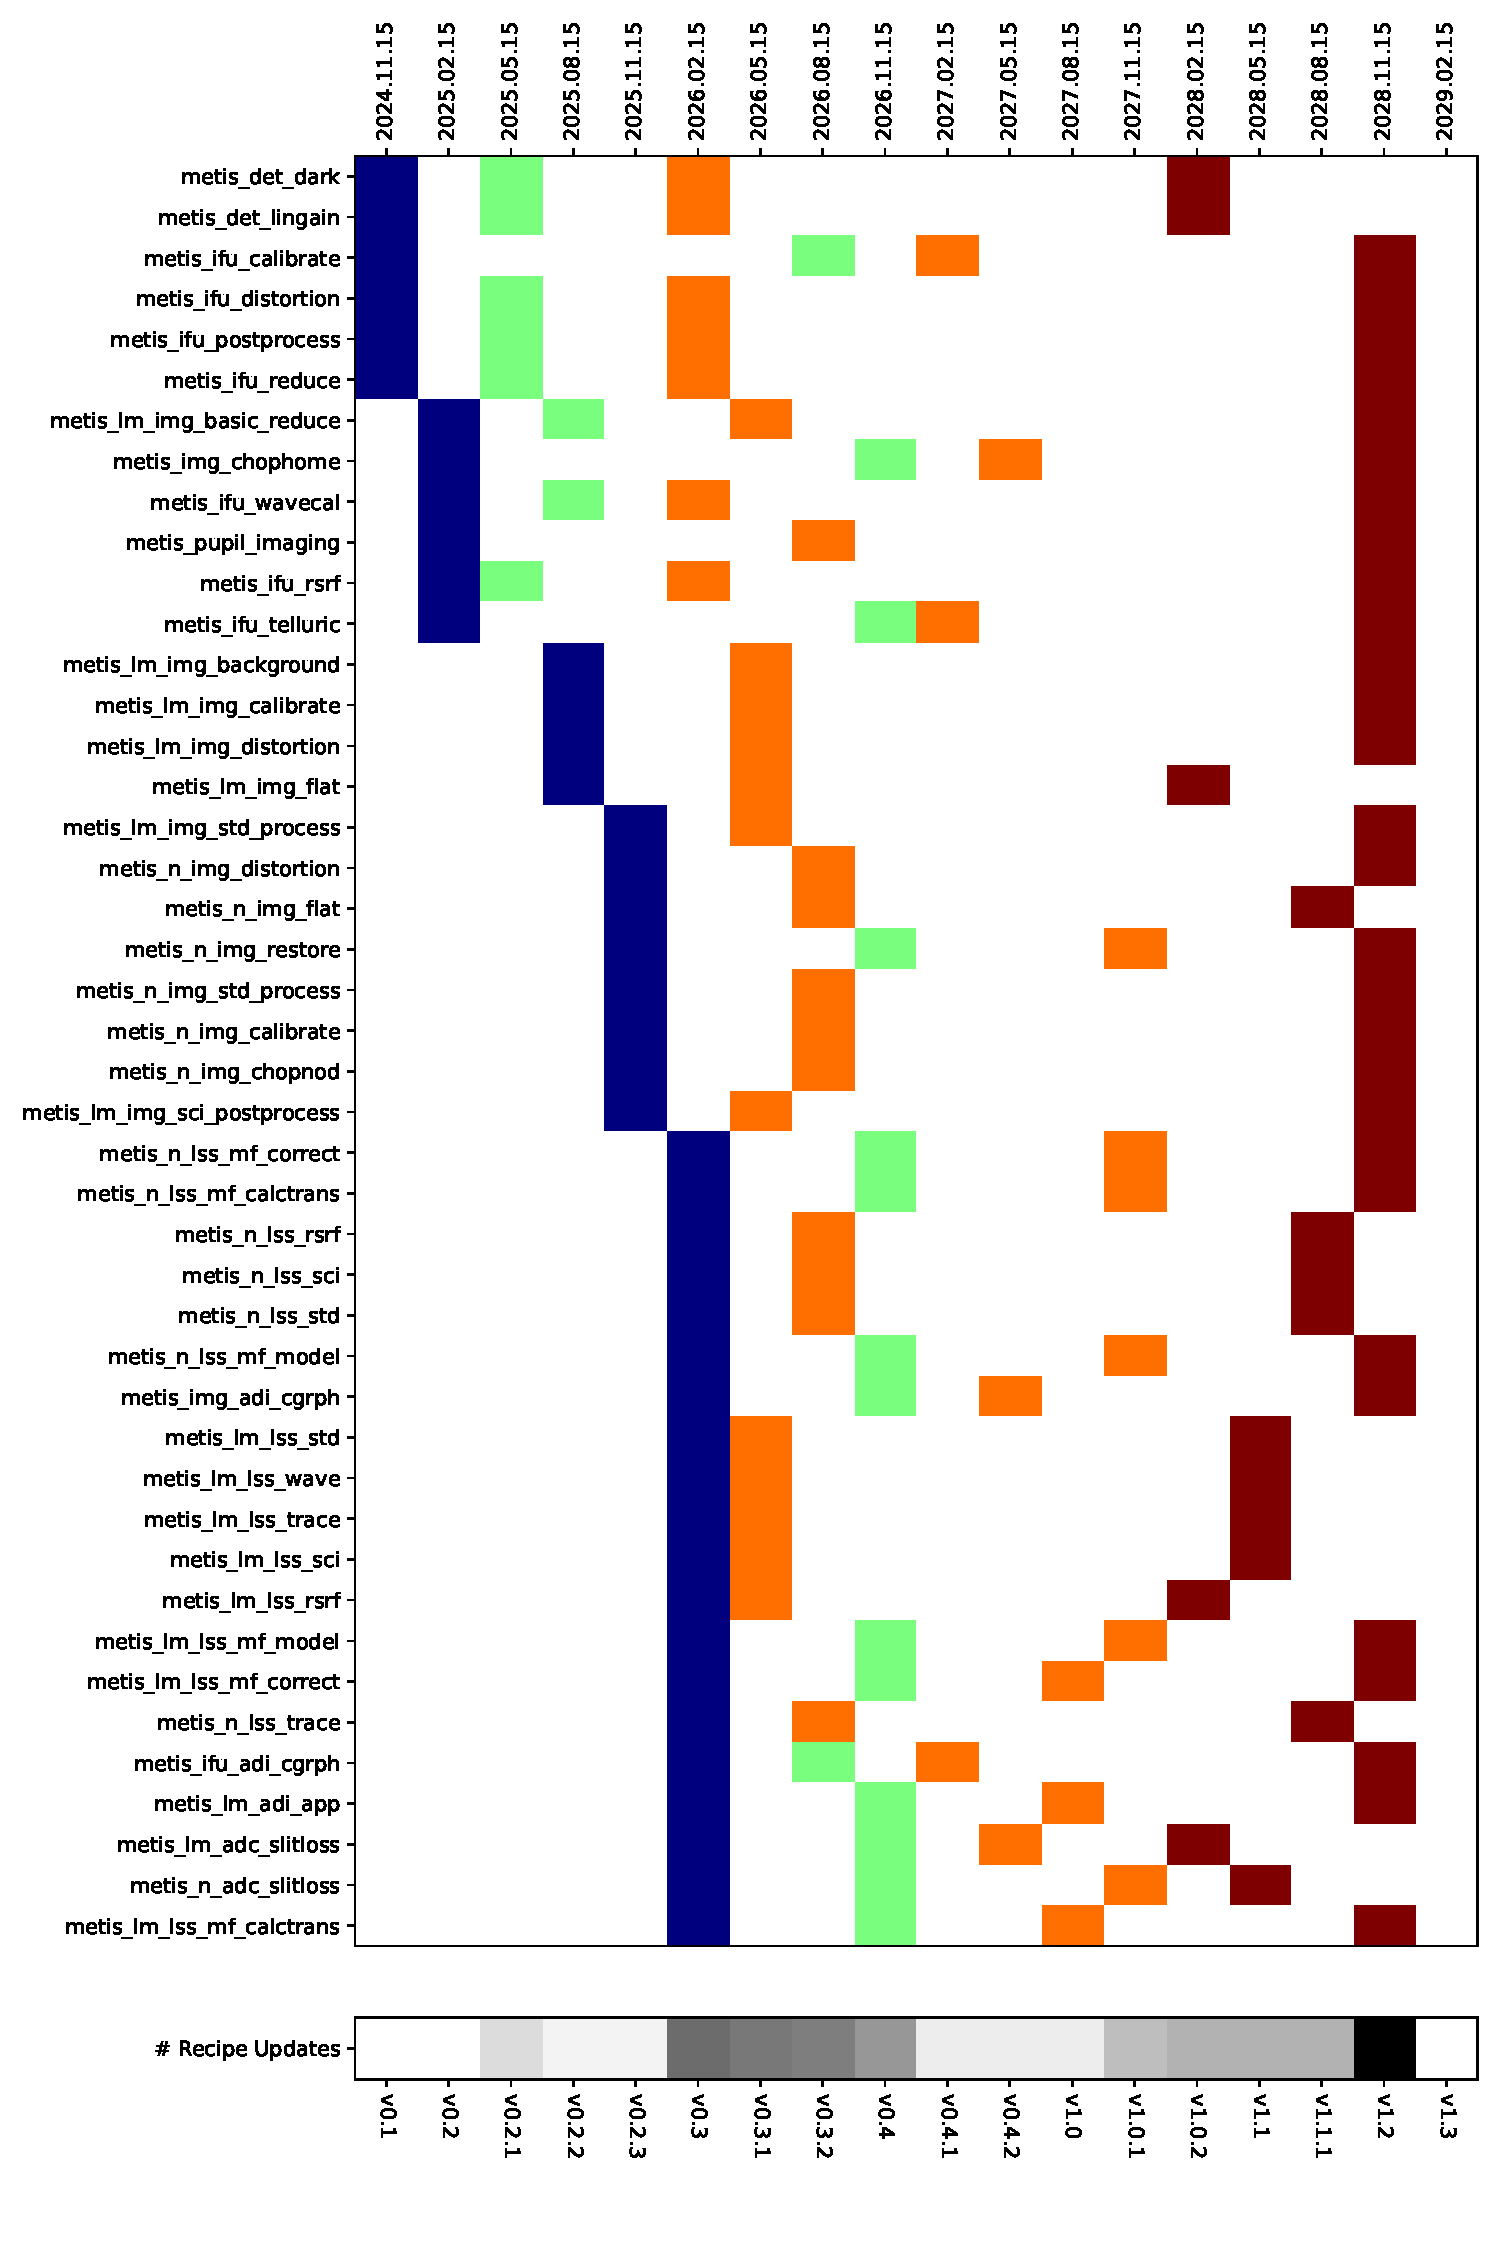
\includegraphics[width=0.83\textwidth]{SPIE_paper/figures/deliveries_recipes.pdf}
    \caption{Current delivery schedule for the METIS pipeline. Every 3 months during the AIV phase of METIS the pipeline team will release an update of the software. The 4 levels of recipe development are represented here thusly: blue = skeleton, green = functional, orange = performance, red = science-grade. The description of functionality for each of the development levels is given in subsection \ref{subsec:imp_levels}.}
    \label{fig:del_schedule}
\end{figure}

\section{Pipeline topology}
\label{sec:pip}

The METIS pipeline team passed the final design review with ESO in November 2023. 





- Association matrices
- See DRL-D + DRL-VT, PIP-FDR success




\section{Outlook until PAE}
\label{sec:outlook}
- Issues on the horizon
- Upcoming milestones


\appendix    %>>>> this command starts appendixes

\acknowledgments % equivalent to \section*{ACKNOWLEDGMENTS}       


% References
\bibliography{report} % bibliography data in report.bib
\bibliographystyle{spiebib} % makes bibtex use spiebib.bst

\end{document} 
